\begin{equation}
    \begin{gathered}
        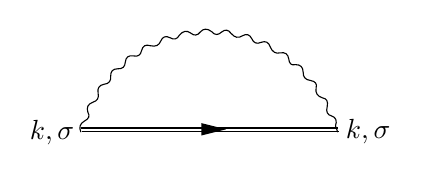
\begin{tikzpicture}[x=0.75pt,y=0.75pt,yscale=-1,xscale=1]
            %uncomment if require: \path (0,300); %set diagram left start at 0, and has height of 300
            
            %Straight Lines [id:da7649384762699059] 
            \draw    (274,238) -- (397.71,238) ;
            %Straight Lines [id:da04845933897994015] 
            \draw    (344,238.62) ;
            \draw [shift={(344,238.62)}, rotate = 180] [fill={rgb, 255:red, 0; green, 0; blue, 0 }  ][line width=0.08]  [draw opacity=0] (12,-3) -- (0,0) -- (12,3) -- cycle    ;
            %Straight Lines [id:da7745729731375024] 
            \draw    (274.74,239.78) -- (398.44,239.78) ;
            %Curve Lines [id:da11998126870239156] 
            \draw    (274,240) .. controls (272.94,237.69) and (273.5,235.91) .. (275.68,234.65) .. controls (277.88,233.56) and (278.44,232.15) .. (277.35,230.42) .. controls (276.59,228.07) and (277.36,226.47) .. (279.66,225.62) .. controls (281.95,224.93) and (282.82,223.43) .. (282.27,221.12) .. controls (281.84,218.75) and (282.81,217.35) .. (285.17,216.92) .. controls (287.5,216.65) and (288.55,215.36) .. (288.34,213.03) .. controls (288.25,210.66) and (289.39,209.47) .. (291.75,209.46) .. controls (294.06,209.59) and (295.27,208.5) .. (295.39,206.2) .. controls (295.64,203.87) and (296.92,202.88) .. (299.23,203.25) .. controls (301.46,203.75) and (302.8,202.88) .. (303.24,200.63) .. controls (303.82,198.38) and (305.21,197.61) .. (307.42,198.34) .. controls (310,198.96) and (311.68,198.2) .. (312.47,196.07) .. controls (313.39,193.94) and (314.87,193.42) .. (316.92,194.49) .. controls (318.87,195.66) and (320.38,195.24) .. (321.46,193.25) .. controls (323.21,191.18) and (325,190.84) .. (326.85,192.23) .. controls (328.58,193.69) and (330.14,193.52) .. (331.52,191.72) .. controls (333.03,189.97) and (334.85,189.92) .. (337,191.57) .. controls (338.48,193.29) and (340.05,193.37) .. (341.7,191.82) .. controls (343.47,190.34) and (345.03,190.54) .. (346.37,192.43) .. controls (348.08,194.46) and (349.88,194.84) .. (351.77,193.59) .. controls (353.78,192.42) and (355.3,192.88) .. (356.33,194.97) .. controls (357.22,197.08) and (358.71,197.66) .. (360.8,196.72) .. controls (362.99,195.9) and (364.45,196.61) .. (365.16,198.84) .. controls (366.19,201.35) and (367.83,202.33) .. (370.08,201.78) .. controls (372.42,201.37) and (373.77,202.35) .. (374.13,204.71) .. controls (374.35,207.05) and (375.43,207.96) .. (377.36,207.44) .. controls (379.78,207.43) and (381.02,208.63) .. (381.07,211.06) .. controls (381,213.46) and (382.16,214.8) .. (384.56,215.07) .. controls (387.01,215.52) and (387.92,216.73) .. (387.29,218.71) .. controls (386.92,221.16) and (387.94,222.73) .. (390.33,223.44) .. controls (392.42,223.74) and (393.2,225.15) .. (392.65,227.68) .. controls (392,230.16) and (392.71,231.66) .. (394.77,232.19) .. controls (396.84,232.82) and (397.48,234.42) .. (396.67,236.99) -- (397.71,240) ;
            
            % Text Node
            \draw (272,240) node [anchor=east] [inner sep=0.75pt]    {$\boldsymbol{k} , \sigma $};
            % Text Node
            \draw (400.44,239.78) node [anchor=west] [inner sep=0.75pt]    {$\boldsymbol{k} , \sigma$};
            \end{tikzpicture}            
    \end{gathered} = \int \frac{\dd[3]{\vb*{q}}}{(2\pi)^3} (- \expval{n_{\vb*{q} \sigma}}) \frac{- \ii 4 \pi e^2}{\abs*{\vb*{k} - \vb*{q}}^2} .
\end{equation}